350. Борис, Виктор, Георгий и Дмитрий играли в игры, ничьих не было. По итогам они частично заполнили таблицу, кто сколько раз у кого выиграл. Если в клетке на пересечении строки Дмитрия и столбца Виктора написано $2:1,$ это значит, что Дмитрий выиграл у Виктора 2 раза и 1 раз ему проиграл. Известно, что Дмитрий проиграл в три раза больше раз, чем выиграл; Виктор выиграл пять раз; Георгий проиграл Дмитрию треть от всех игр между ними; Борис проиграл каждому одинаковое число раз. Сколько раз Дмитрий проиграл Борису? Заполните целиком таблицу ниже.\\
\begin{figure}[ht!]
\center{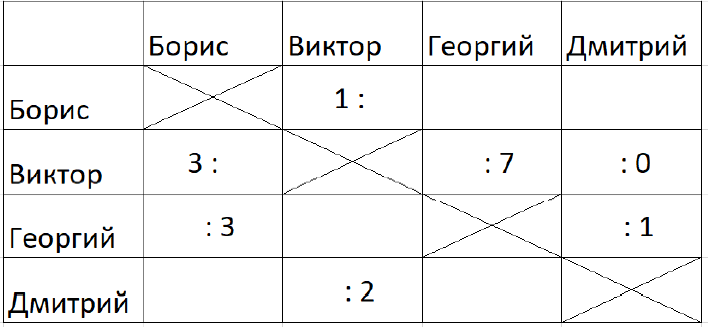
\includegraphics[scale=0.35]{tab4.png}}
\end{figure}\\
